\section{Implementation results}
\label{sec:results}

\subsection{Test performance and model size}
\label{sec:quantitative}
\reporttodo{Add one table of test accuracy, macro-F1, and trainable parameters.
Identify the dataset, seed count, training budget, and selected checkpoints.
Check every value against its result JSON. Compare timing only under a documented,
comparable protocol.}

\subsection{Learning behavior}
\reporttodo{Compare architectures in one learning-curve figure per dataset.
Discuss convergence, instability, train--validation gaps, and checkpoint choice
where the curves support those observations. Note relevant implementation issues.}

\subsection{Per-class performance and error analysis}
\label{sec:errors}

The analysis uses the official Fashion-MNIST test set of 10,000 images, with
1,000 images per class. Table~\ref{tab:class-recall} reports class recall for five
architectures, each trained for 50 epochs with seed 42. Checkpoints were selected
by validation loss. For the detailed comparison, we select the MLP as the
flattened-pixel baseline because its minimum validation loss is lower than that
of the linear classifier, 0.3413 against 0.6540. We compare this baseline with the
CNN without using test performance to select the baseline.

\begin{table}[htbp]
\centering\small
\caption{Fashion-MNIST test recall by class, in percent. Each class contains
1,000 test images. All entries refer to seed 42 and validation-selected checkpoints
from 50-epoch runs.}
\label{tab:class-recall}
\begin{tabular}{lrrrrr}
\toprule
Class & Linear & MLP & CNN & GRU & Transformer\\\midrule
T-shirt/top & 75.5 & 84.4 & 86.7 & 85.1 & 81.8\\
Trouser & 90.7 & 97.0 & 96.2 & 97.3 & 98.0\\
Pullover & 62.8 & 79.8 & 86.3 & 81.6 & 84.0\\
Dress & 77.0 & 87.5 & 80.3 & 89.5 & 93.2\\
Coat & 68.1 & 79.7 & 67.8 & 85.4 & 85.6\\
Sandal & 89.0 & 95.3 & 96.5 & 96.7 & 96.6\\
Shirt & 40.3 & 62.1 & 59.6 & 72.4 & 72.3\\
Sneaker & 84.4 & 93.7 & 95.8 & 95.5 & 97.2\\
Bag & 89.2 & 97.1 & 97.4 & 98.1 & 98.7\\
Ankle boot & 93.5 & 95.2 & 95.5 & 97.2 & 96.9\\
\bottomrule
\end{tabular}
\end{table}


\paragraph{Distribution of errors.}
Shirt has the lowest recall for every model in Table~\ref{tab:class-recall}.
Its recall increases from 40.3\% for the linear classifier to 62.1\% for the MLP,
72.4\% for GRU, and 72.3\% for the Transformer. CNN attains 59.6\%.
The difficulty therefore persists across representations, although its extent
varies. By contrast, Bag recall lies between 97.1\% and 98.7\% for the four
nonlinear models. Aggregate accuracy conceals this difference between classes.

Figure~\ref{fig:paired-confusion} shows the directional errors of MLP and CNN.
Of the 1,000 Shirt images, MLP assigns 179 to T-shirt/top, whereas CNN assigns
191. Coat is another substantial source of disagreement. CNN assigns 175 Coat
images to Pullover and 112 to Shirt, and correctly identifies 67.8\% of Coat
images. MLP assigns 96 Coat images to Pullover and achieves 79.7\% Coat recall.
CNN improves Pullover recall from 79.8\% to 86.3\%, but reduces Coat recall by
11.9 percentage points. Its effect is thus class-dependent.

\begin{figure}[htbp]
\centering
\begin{minipage}[t]{0.49\linewidth}
\centering
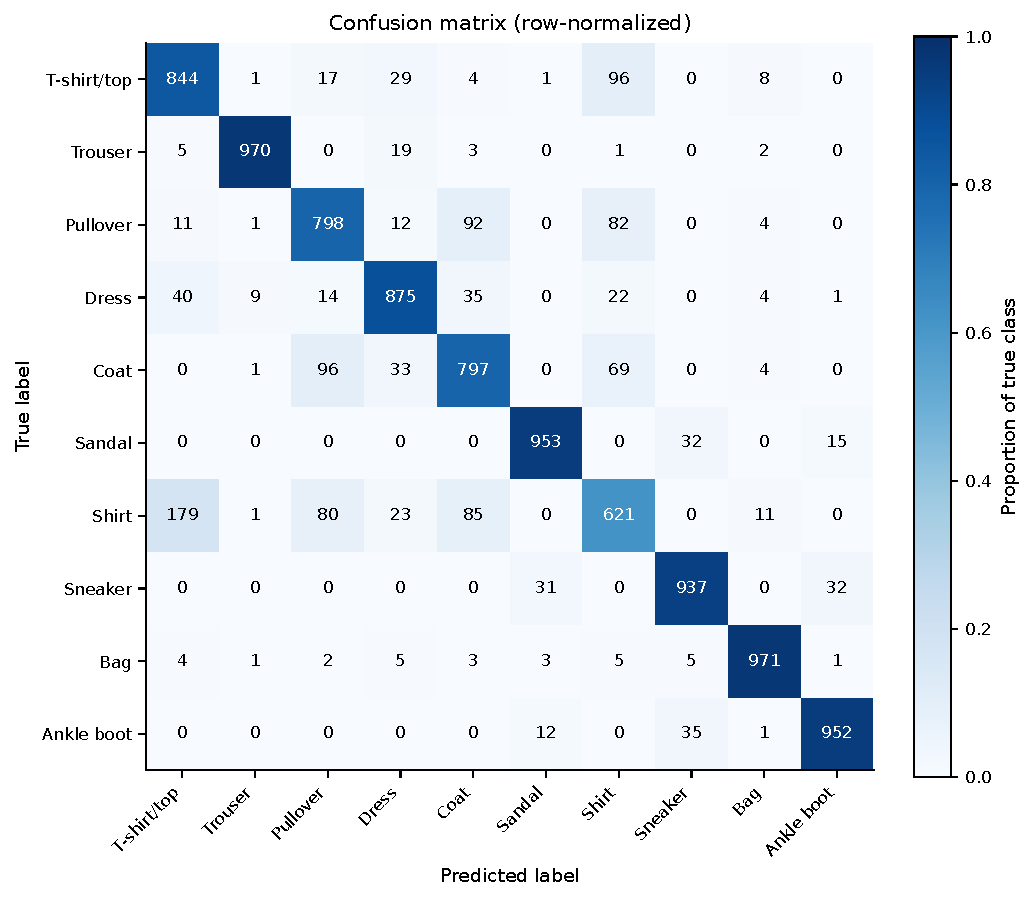
\includegraphics[width=\linewidth]{Images/fashion_mnist_mlp_confusion.pdf}
\par\small (a) MLP
\end{minipage}\hfill
\begin{minipage}[t]{0.49\linewidth}
\centering
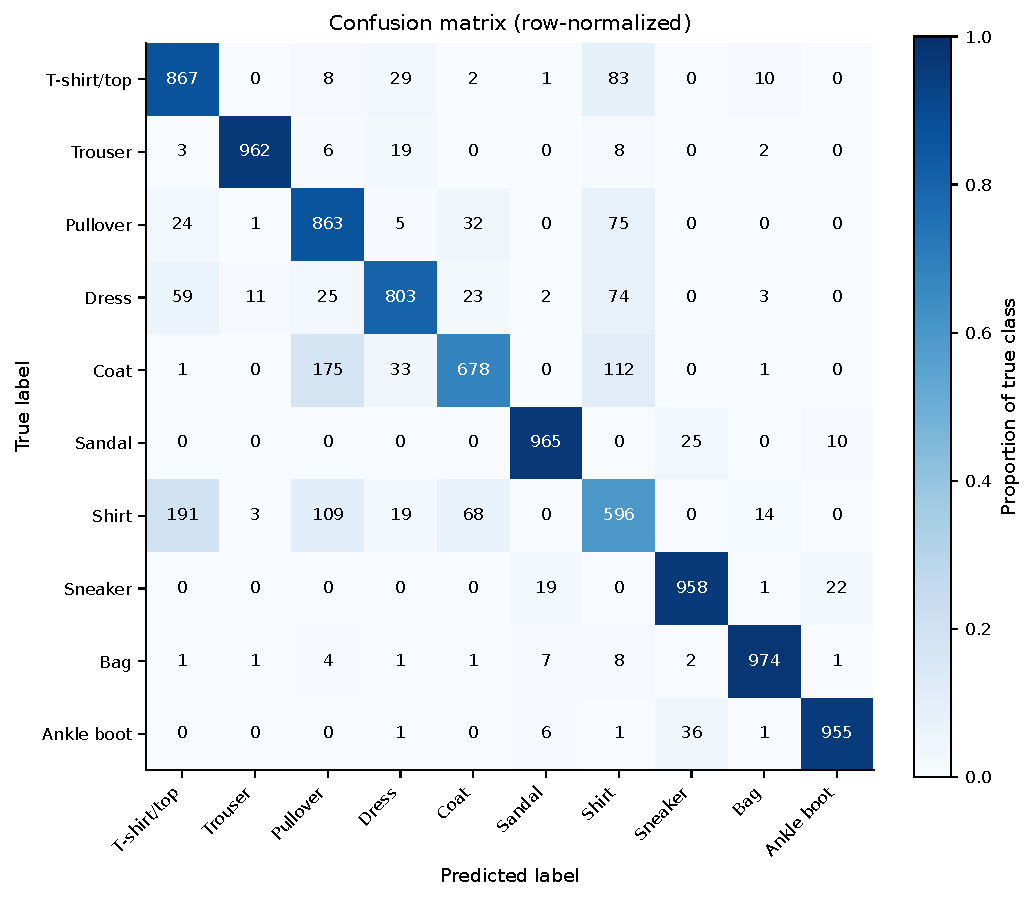
\includegraphics[width=\linewidth]{Images/fashion_mnist_cnn_confusion.pdf}
\par\small (b) CNN
\end{minipage}
\caption{Fashion-MNIST test confusion matrices. Rows denote true classes and
columns predicted classes. Color gives the proportion within each true class;
cell annotations give counts. Both panels use the same color scale.}
\label{fig:paired-confusion}
\end{figure}

Errors between T-shirt/top, Pullover, Coat, and Shirt account for 811 of the
MLP's 1,282 mistakes, 63.3\%, and 880 of the CNN's 1,379 mistakes, 63.8\%.
Here, an error belongs to this group only when both its true and predicted
labels are among these four classes. Similar garment outlines offer a plausible
explanation for this concentration. The comparison does not isolate that
explanation, nor establish that flattening causes the errors. In particular,
convolution does not remove the dominant confusions in this configuration.

\subsection{Predictions on shared images}
\label{sec:qualitative}

Across the complete test set, CNN correctly classifies 532 images that MLP
misclassifies. Conversely, MLP correctly classifies 629 images that CNN
misclassifies. Both models err on 750 images and correctly classify 8,089.
The difference between the two disagreement counts gives CNN 97 additional
errors, consistent with its 0.97-percentage-point accuracy deficit. Neither
model's correct predictions contain all those of the other.

Figure~\ref{fig:shared-predictions} illustrates these three error categories.
Within each category, we take the first two examples in official test-set order.
Indices are zero-based. The selection is deterministic, but the equal number of
examples per category does not represent their relative frequencies. Predictions
from all five architectures are shown for each selected image.

\begin{figure}[htbp]
\centering
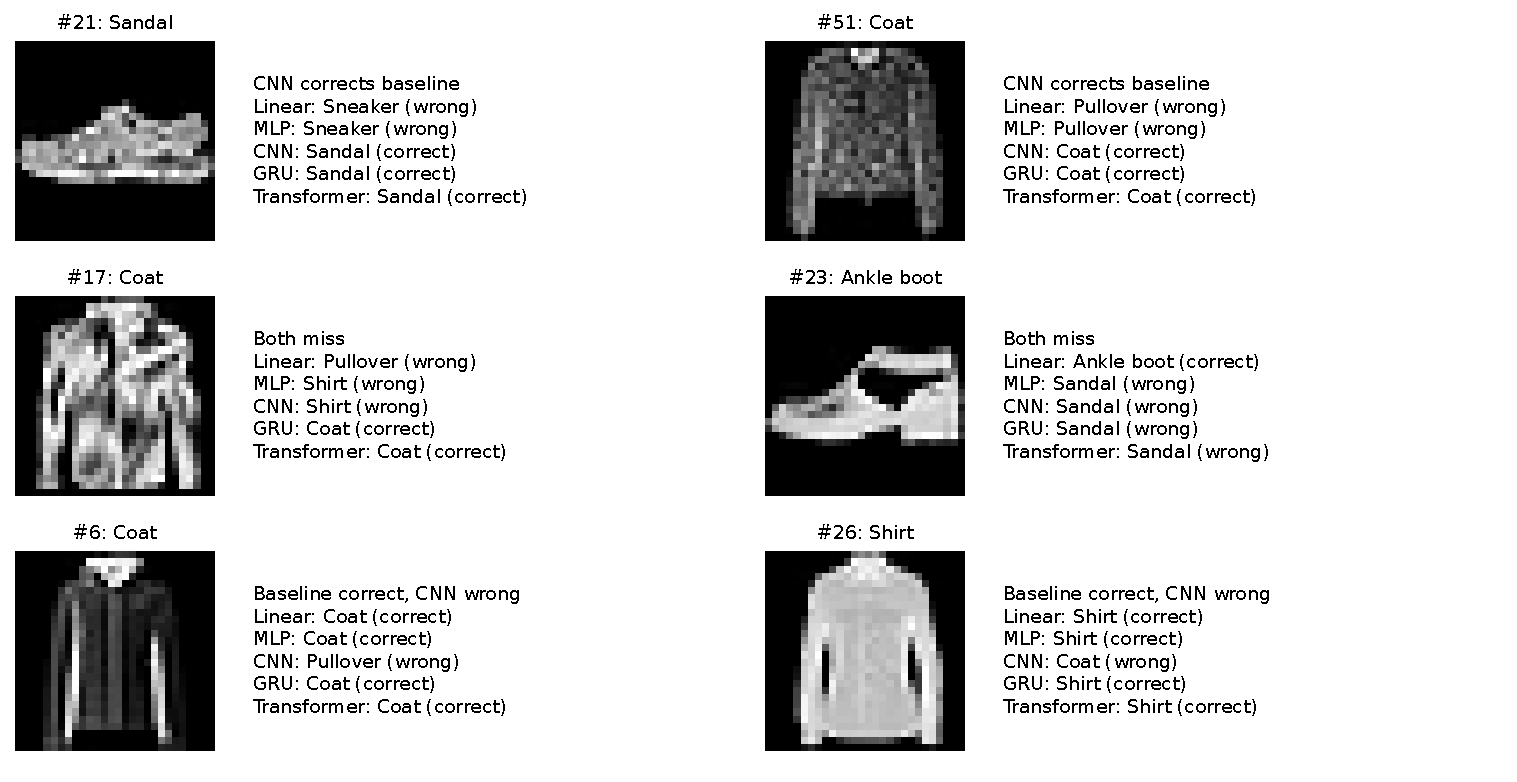
\includegraphics[width=\linewidth]{Images/fashion_mnist_shared_images.pdf}
\caption{Shared Fashion-MNIST test images with their true labels and model
predictions. Each row contains two examples from one category: CNN corrects an
MLP error; both models err; MLP is correct and CNN errs. ``Baseline'' denotes MLP.
The displayed indices specify the examples independently of their appearance.}
\label{fig:shared-predictions}
\end{figure}

For Coat image 51, both flattened-pixel models predict Pullover, while CNN,
GRU, and Transformer predict Coat. For Coat image 6, however, MLP is correct
and CNN predicts Pullover. The same pair of classes therefore contributes errors
in both disagreement directions. Image 17 provides a further distinction:
MLP and CNN predict Shirt for a Coat that GRU and Transformer classify correctly.
In image 23, only the linear classifier identifies Ankle boot; all four nonlinear
models predict Sandal. These examples illustrate differences in individual
predictions and do not establish general superiority of any architecture.

The measured errors suggest a focused follow-up: examine the garment pairs
under a controlled change in spatial representation or augmentation, with the
remaining training settings fixed and several seeds. Such an experiment would
test a proposed explanation for the confusions. The present observations alone
do not determine their cause. Likewise, confidence on selected mistakes cannot
establish calibration without a separate analysis of predicted probabilities.

\subsection{Architecture trade-offs}
\label{sec:discussion}
\reporttodo{Answer the research question with measured differences in quality,
model size, and verified compute cost. Discuss representation and inductive bias
without claiming a causal explanation that the experiment did not test.}

\subsection{Additional experiments}
\reporttodo{Report completed ablations or extensions separately, with their
controls and findings. Remove this subsection if no additional experiment belongs here.}

\subsection{Limitations}
\reporttodo{State the limits from seed count, tuning, unequal budgets, timing,
and dataset representativeness. Explain which conclusions the evidence cannot support.}

\subsection{Conclusion}
\reporttodo{Give a short answer to the research question and the practical
trade-off supported by the results. End with one useful next experiment.}
